\documentclass{rapport}
\usepackage{pythontex}
\usepackage{csquotes}
\addbibresource{library.bib}


\begin{document}

%----------- Informations du rapport ---------

\unif{HEIG-VD}
\titre{Mini-projet} %Titre du fichier .pdf
\cours{Capteurs} %cours
\sujet{Capteur de proximité inductif} %Nom du sujet
%\groupe{Groupe} %Nom du groupe  

\enseignant{Michel  \textsc{Demierre} 
        } %Nom de l'enseignant

\eleves{Bianchi   \textsc{ Romain} \\
Larghi  \textsc{ Andrea}
         } %Nom des élèves

\nom{Bianchi Romain, Larghi Andrea} %nom dans l'entête

%----------- Initialisation -------------------


\fairepagedegarde %Créer la page de garde
\thispagestyle{noPage}
\tabledematieres %Créer la table de matières
\thispagestyle{noPage}
\newpage
\listoffigures
\listoftables
\clearpage
\setcounter{page}{1}
\fairemarges %Afficher les marges
%------------ Corps du rapport ----------------


\begin{pycode}
    
\end{pycode}

\section{Introduction}

Dans le cadre du cours "Capteurs", trois séances de laboratoires portant
sur l'étude du comportement d'un capteur inductif à courant de Foucault ont été effectuées. 
Ce document présent est un rapport intermédiaire de ce mini-projet répondant aux objectifs.

\subsection{Objectifs}

\begin{itemize}
    \item Appliquer les connaissances acquises au cours ;
    \item Observer comment se comportent la résistance et l'inductance du capteur ;
    \item Optimiser la sensibilité du capteur ;
    \item Déterminer la fonction de transfert et la transformée de Möbius. 
\end{itemize}

\subsection{Matériel}

\begin{table}[H]
    \centering
    \begin{tabular}{|c|c|c|c|}
    \hline
    \textbf{Nom}          & \textbf{Marque} & \textbf{Modèle} & \textbf{N° de série} \\ \hline
    Capteur (maquette)    & -               & HEIG-VD         & 09                   \\ \hline
    Circuit imprimé       & -               & HEIG-VD         & 12                   \\ \hline
    Boite de laboratoire  & -               & HEIG-VD         & 1                    \\ \hline
    Multimètre            & Keysight        & 34460A          & MY53102179           \\ \hline
    Oscilloscope          & Tektronix       & DPO 2014B       & C030007              \\ \hline
    Générateur de signal  & SIGLENT         & SDG2082X        & SDG"XCA1160916       \\ \hline
    Générateur de tension & GWINSTEK        & GPD-3303S       & A140629              \\ \hline
    Analyseur d'impédance & Keysight        & E4990A          & MY54100421           \\ \hline
    \end{tabular}
    \caption{Liste du matériel}
    \end{table}





    


\begin{pycode}



\end{pycode}

\section{Séance 1 - Caractéristique de la bobine }

\subsection{Objectifs}

Le but de cette première séance est de caractériser l'impédance du capteur en fonction de la distance
à laquelle se trouve la cible.

%de caractériser le capteur de proximité inductif à travers 
%l’analyse de la résistance et l'inductance de la bobine, en fonction de la distance cible-capteur 
% et de la fréquence. 

\subsection{Méthode}

\begin{enumerate}
    \item Brancher la maquette sur l'analyseur d'impédance comme montré ci-dessous (cf. fig. \ref{fig: AI});
    \item Déterminer la distance de butée et se positionner à 0.5 mm de celle-ci ;
    \item Enregistrer la mesure de l'appareil qui permet d'obtenir la résistance ainsi que l'inductance de 
    la bobine sur un intervalle de 100 kHz à 15 MHz ;
    \item Répéter l'opération par pas de 0.05 mm jusqu'à atteindre 0.90 mm ce qui totalise 9 mesures.
\end{enumerate}

\insererfigure{Images/Seance1/AnalyseurImpedance.jpg}{6cm}{analyseur d'impédance}{AI}

\subsection{Caractérisation de la bobine}

\subsubsection{Impédance}


Les mesures réalisées avec l'analyseur d'impédance ont été sauvegardées en un total
de 9 fichiers CSV, un pour chacune des distances. Chaque fichier comporte une colonne propre à
la fréquence, l'inductance et la résistance. Ainsi, il est possible de déterminer l'impédance, relative
à la fréquence, selon les 9 positions de la bobine.\\


Impédance de la bobine : 

\begin{equation}
    Z_b = R_b + j \omega L_b
\end{equation}

Avec : \\
$Z_b$, l'impédance de la bobine [$\Omega$];\\
$R_b$, la résistance de la bobine [$\Omega$];\\
$L_b$, l'inductance de la bobine;\\
$\omega$, la pulsation = $ 2 \cdot \pi \cdot f$ [rad/s] ;\\
f, la fréquence [Hz].\\

Représentations schématiques du circuit : 

\begin{figure}[H]
    \begin{minipage}[c]{.50\linewidth}
        \centering
        \rotatebox{0}{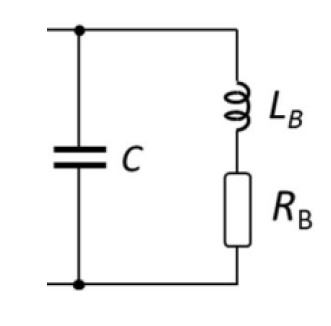
\includegraphics[scale=0.6]{Images/Seance1/Sch1.jpg}}
        \caption{Schéma électrique en série }
    \label{fig:SCH1}
    \end{minipage}
    \hfill%
    \begin{minipage}[c]{.50\linewidth}
        \centering
        \rotatebox{0}{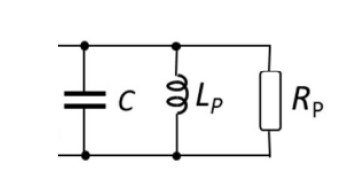
\includegraphics[scale=0.9]{Images/Seance1/Sch2.jpg}}
        \caption{Schéma électrique en parallèle }
    \label{fig:SCH2}
    \end{minipage}
\end{figure}

L'impédance ainsi déterminée a permis de représenter graphiquement l'inductance et la résistance de 
la bobine en fonction de la fréquence :


\insererfigure{Images/Seance1/Lf2.png}{8cm}{Inductance en fonction de la fréquence}{Lf}
\insererfigure{Images/Seance1/Rf2.png}{8cm}{Résistances en fonction de la fréquence}{Rf}

L'allure des courbes représentées sur les graphiques (cf. fig. \ref{fig: Lf} et \ref{fig: Rf})
correspondent au comportement d'un circuit RLC. Ce résultat est représentatif du montage étudié.
En effet, la \textbf{R}ésistance et est celle du fil de la bobine, l'inductance \textbf{L} est celle 
de la bobine, le \textbf{C}ondensateur est la capacité relative à la 
cible et à sa distance.\\

La fréquence de résonance du circuit peut-être aisément relevée puis-ce qu'il s'agit du passage à 0 
de l'inductance et le pic de résistance. On relève graphiquement à la 
position de repos une fréquence de résonance de 6.77 Mhz. La figure \ref{fig: Lf} montre encore
qu'à basse fréquence l'inductance est constante ce qui suggère la présence d'une cible non-ferromagnétique\\

%La figure \ref{fig: Rf} montre que les courbes se croisent à 1.63 MHz. 

%On note encore que les courbes de résistance
%se croisent à 1.62 MHz ce qui représente l'en\\


%\begin{figure}[H]
%    \begin{minipage}[c]{.50\linewidth}
 %       \centering
  %      \rotatebox{0}{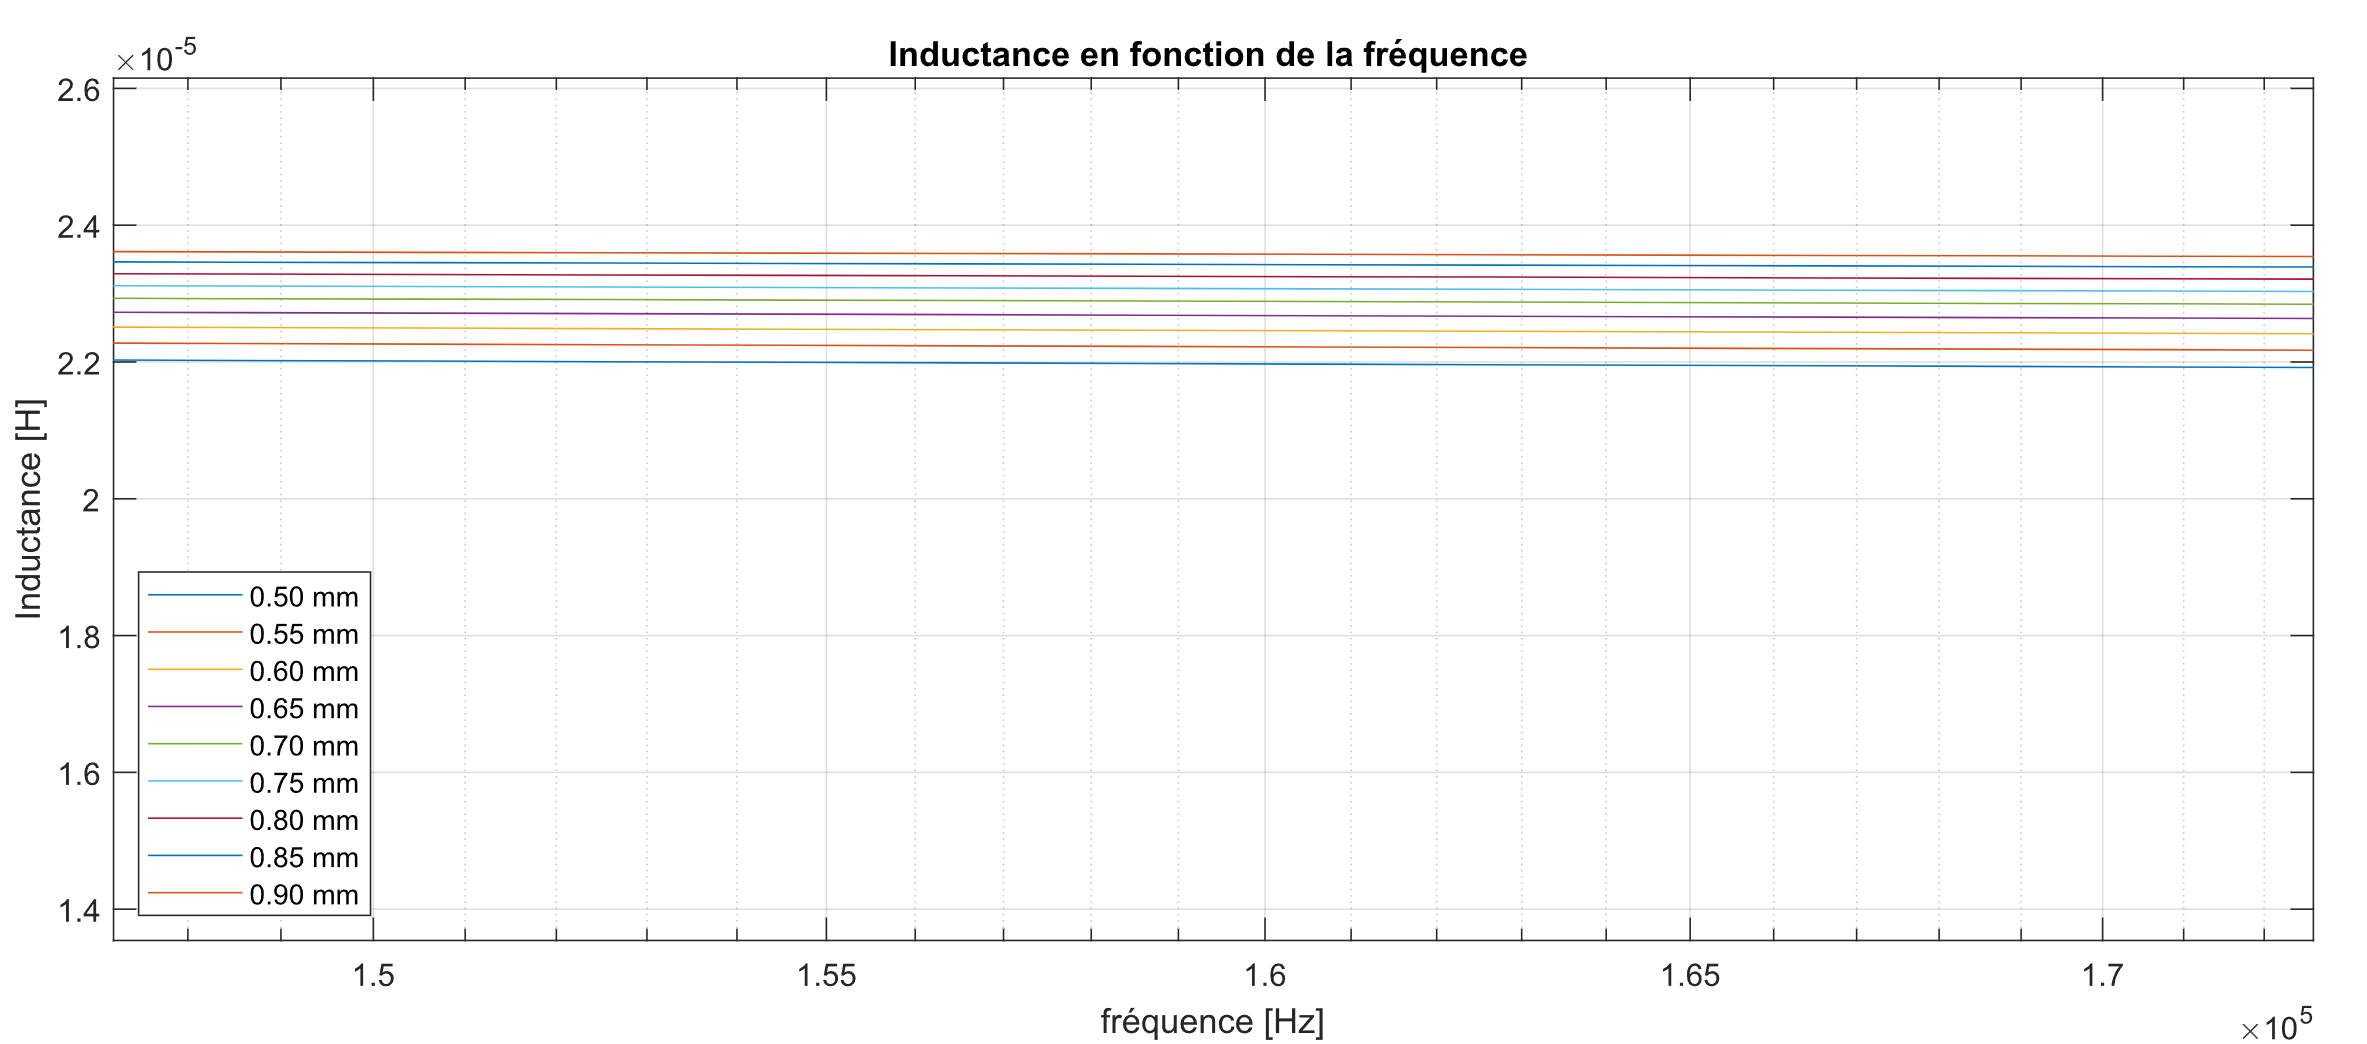
\includegraphics[scale=0.2]{Images/Seance1/zoom1L.png}}
  %      \caption{Zoom sur la figure \ref{fig: Lf}}
  %  \label{fig:SCH3}
  %  \end{minipage}
  %  \hfill%
  %  \begin{minipage}[c]{.50\linewidth}
  %      \centering
  %      \rotatebox{0}{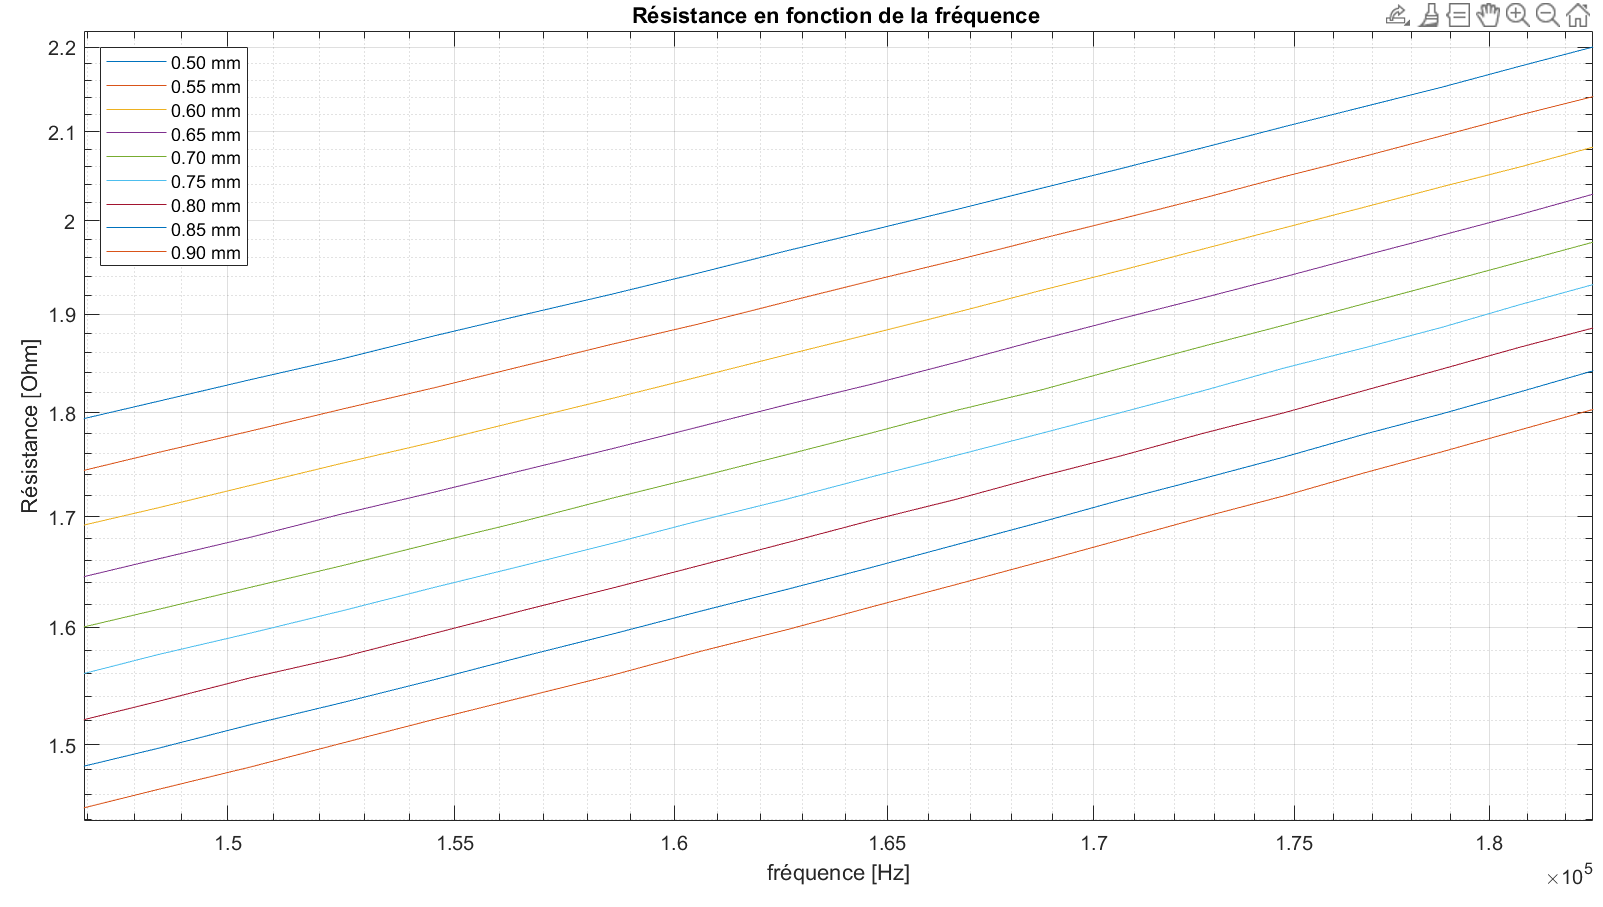
\includegraphics[scale=0.2]{Images/Seance1/zoom2R.png}}
  %     \caption{Zoom sur la figure \ref{fig: Rf}}
 %\label{fig:SCH4}
 %   \end{minipage}
%\end{figure}

Il est enfin possible de constater qu'en basses fréquences (140-160 kHz) les différentes courbes évoluent
de manière linéaire. \\





L'inductance et la résistance à 150 kHz en fonction de la distance ont ensuite été représentées :

\insererfigure{Images/Seance1/Lx.png}{8cm}{Inductance en fonction de la distance}{Lx}
\insererfigure{Images/Seance1/Rx.png}{8cm}{Résistances en fonction de la distance}{Rx}

Les courbes tracées permettent de déterminer le type de matériau de la cible, ferromagnétique ou 
non-ferromagnétique. Les figures \ref{fig: Lx} et \ref{fig: Rx} montrent une augmentation de 
l'inductance et une diminution de la résistance lors de l'éloignement de la cible ce qui correspond 
au comportement d'un matériau conducteur non-ferromagnétique. 
De plus, la cible est de couleur orangée et comportant des marques d'oxydation, ce qui permet 
de conclure qu'elle est en \textbf{cuivre}.\\  

%Les régressions réalisées (cf. fig. \ref{fig: Lx} et \ref{fig: Rx}) 


L'impédance de la bobine aux différentes distrances pour une fréquence de 150kHz à finalement été tracée :

\insererfigure{Images/Seance1/Zx.png}{8cm}{Impédance de la bobine aux distances}{Zx}

La figure \ref{fig: Zx} montre que l'impédance évolue de manière "quasi" linéaire, avec un coefficient 
de détermination $R^2$ = 0.9999. On remarque toute fois que la distance entre les point ne sont pas les mêmes. 
Plus la cible s'éloigne, plus les points se rapprochent et la sensibilité diminue (eq :\ref{eq:s}).
Ceci montre les limites de ce système, car si la sensibilité est trop faible alors les valeurs relevées
ne sont plus détectables.
\subsubsection{Sensibilité}

Grâce aux valeurs relevées, il est également possible de déterminer la sensibilité de
ce capteur qui, pour une position de repos à 0.7 mm s'exprime : 

\begin{equation}\label{eq:s}
    \left . S_b \right |_{x=0.7} = \left . \frac{\left | \delta \underline{Z_b}\right |}{\delta x} \right |_{x=0.7}
\end{equation}

Avec: \\
$S_b$, la sensibilité [$\Omega/mm$];\\
$\delta Z$, l'écart d'impédance = $Z_{0.75} - Z_{0.65}$ [$\Omega$];\\
$\delta x$, l'écart de distance  = $x_{0.75} - x_{0.65}$ [mm].



\insererfigure{Images/Seance1/Sensi.png}{8cm}{Sensibilité en fonction de la fréquence}{S}

Le graphique ci-dessus montre la sensibilité calculée avec l'équation \ref{eq:s} en fonction
de la fréquence, pour une position de repos de 0.7mm. Cette représentation permet d'observer
qu'un pic sensibilité se forme de 5 à 9 MHz, culminant à 21'235 [$\Omega$/mm] à la fréquence 
de 6.78 MHz. 

 
\subsection{Conclusion}

Les premières analyses de ce capteur ont donné des résultats cohérents et qui permettent
d'avoir une bonne appréhension des prochaines séances.\\

Résumer des résultats :

\begin{enumerate}
    \item Le matériau constituant la cible est le cuivre;
    \begin{itemize}
        \item Comportement conducteur non-ferromagnétique;
        \item Couleur orangée.
    \end{itemize}
    \item Pour une fréquence de 150 kHz on observe une progression linéaire de l'impédance en selon
    la position de la cible;
    \item La fréquence de résonance du capteur est de 6.78 MHz;
    \begin{itemize}
        \item Passage à 0 de l'inductance et pic de résistance (cf. fig. \ref{fig: Lf} et \ref{fig: Rx})
        \item Pic de sensibilité (cf. fig. \ref{fig: S}). 
    \end{itemize}
\end{enumerate}


\begin{pycode}

\end{pycode}

\section{Séance 2 - Fréquence de résonance et fonction de transfert}


\subsection{Objectifs}

\subsection{Méthode}

\subsection{Résultats}

\subsection{Analyse}

\subsection{Conclusion}

\begin{pycode}

\end{pycode}


\section{Séance 3 - Caractérisation du démodulateur seul}

\subsection{Objectifs}

    L'objectif de la séance est d'observer le comportement du démodulatieur par le biais du
    multiplicateur et du filtre passe-bas ;

    \insererfigure{Images/Seance3/Schs3.jpg}{5cm}{Schéma avec multiplicateur et filtre}{Sch3s}
  

\subsection{Théorie}

\subsubsection{Le multiplicateur}

\insererfigure{Images/Seance3/Mult.jpg}{3cm}{Schéma du multiplicateur}{Mult}

Comme montré sur le schéma ci-dessus (cf. fig. \ref{fig: Mult}), le rôle du multiplicateur
est de multiplier le signal $U_{mod}$ par la valeur du sélecteur. La sélection se fait par l'envoi
d'un signal carré $U_p$ vers le sélecteur qui prend la valeur :

\begin{itemize}
    \item A : +1 quand l'amplitude max du signal est maximale;
    \item B : -1 quand l'amplitude du signal carré est nulle 
\end{itemize}

\subsubsection{Le filtre}

Les filtres passe-bas a plusieurs utilités :

\begin{itemize}
    \item Il supprime la composante 2$f_0$ provenant de la multiplication;\\
   $ A \sin(\omega t) \cdot \sin(\omega t) = \frac{A}{2} \left( \cos(\varphi) - \cos(2\omega t + \varphi) \right)$
    \item Il supprimes des harmoniques du signal carré;
    \item Il diminue du bruit en ne laissant que la bande passante utile.
    
\end{itemize}



\subsection{Méthode}

\subsubsection{Multiplicateur}
\begin{itemize}
    \item Montage :
    \begin{itemize}
        \item Le jumper J6 doit être monté;
        \item Le jumper J3 doit être positionné sur les pins 2 et 3 du PCB;
        \item Brancher la sortie $U_{mult}$ à l'oscilloscope;
        \item Alimenter le PCB à -12 et 12 V;
        \item Alimenter $U_{mod}'$ avec un sinus 1 Vp;
        \item Alimenter $U_{p}$ avec un signal carré 0-5 V.
    \end{itemize}

    \insererfigure{Images/Seance3/Mt2.jpg}{5cm}{Montage réalisé}{Mt}

    \item Mesures :
    \begin{enumerate}
        \item Régler le signal $U_{mod}'$ à 100 kHz;
        \item Faire varier le déphasage de $U_{p}$ de 0 à 180° par pas de 20°;
        \item Réeffectuer l'étape 2 pour une fréquence  $U_{mod}'$ de 300 kHz.
    \end{enumerate}

\end{itemize}

\subsubsection{Filtrage}

\begin{itemize}
    \item Montage :
    \begin{itemize}
        \item Réaliser le montage du filtre ci-dessous;
        \item $R_{14}$ = 0 et $C_6$ = nc;
        \item $R_{10}$ = $R_{13}$ = $\approx$ 10 k$\Omega$.
    \end{itemize}

    \insererfigure{Images/Seance3/Filtre.jpg}{4cm}{Filtre RC}{Filtre}
Il serait possible d'obtenir un filtre d'ordre 2, il suffit de rajouter une capacité $C_6$ de 10 nF.\\

    \item Mesures :
    \begin{enumerate}
        \item Relever la tension $U_{out}$ du démodulateur sur le multimètre, pour les mêmes déphasages
        que pour la manipulation précédente.
        
    \end{enumerate}
\end{itemize}

\subsection{Multiplicateur}

Cette section présente les captures des signaux observés à l'oscilloscope. Il a été décidé de
ne montrer que les déphasages de 0° 60° 120° et 180° afin de ne pas surcharger le rapport.
 Sur les représentations, \textcolor{blue}{$U_{mult}$} est sur le channel 2, 
 \textcolor{magenta}{$U_{mod}'$} le 3 et \textcolor{green}{$U_{p}$} sur le 4. 

\subsubsection{Fréquence de 100 kHz}



\begin{figure}[H]
    \begin{minipage}[c]{.50\linewidth}
        \centering
        \rotatebox{0}{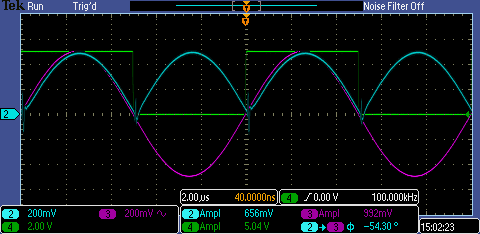
\includegraphics[scale=0.4]{Images/Seance3/partie1/TEK00000.PNG}}
        \caption{$U_{p}$, $U_{mod}'$ et $U_{mult}$ avec un\\ déphasage de 0° à 100 kHz }
    \label{fig:oc11}
    \end{minipage}
    \hfill%
    \begin{minipage}[c]{.50\linewidth}
        \centering
        \rotatebox{0}{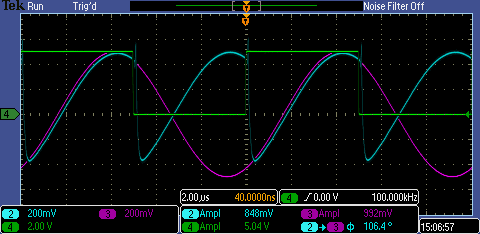
\includegraphics[scale=0.4]{Images/Seance3/partie1/TEK00003.PNG}}
       \caption{$U_{p}$, $U_{mod}'$ et $U_{mult}$ avec un \\ déphasage de 60° à 100 kHz}
 \label{fig:oc12}
    \end{minipage}
\end{figure}

\begin{figure}[H]
    \begin{minipage}[c]{.50\linewidth}
        \centering
        \rotatebox{0}{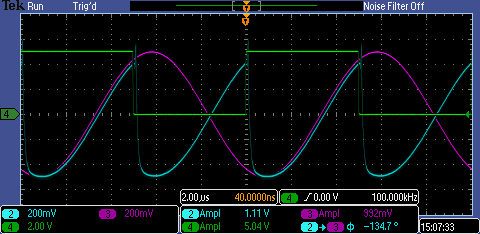
\includegraphics[scale=0.4]{Images/Seance3/partie1/TEK00006.PNG}}
        \caption{$U_{p}$, $U_{mod}'$ et $U_{mult}$ avec un\\ déphasage de 120° à 100 kHz }
    \label{fig:oc13}
    \end{minipage}
    \hfill%
    \begin{minipage}[c]{.50\linewidth}
        \centering
        \rotatebox{0}{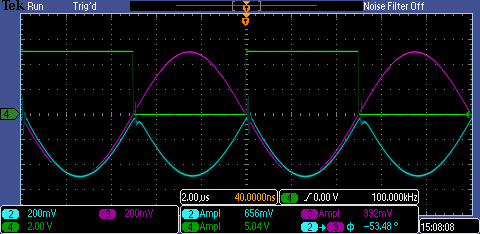
\includegraphics[scale=0.4]{Images/Seance3/partie1/TEK00009.PNG}}
       \caption{$U_{p}$, $U_{mod}'$ et $U_{mult}$ avec un \\ déphasage de 180° à 100 kHz}
 \label{fig:oc14}
    \end{minipage}
\end{figure}


\subsubsection{Fréquence de 300 kHz}


\begin{figure}[H]
    \begin{minipage}[c]{.50\linewidth}
        \centering
        \rotatebox{0}{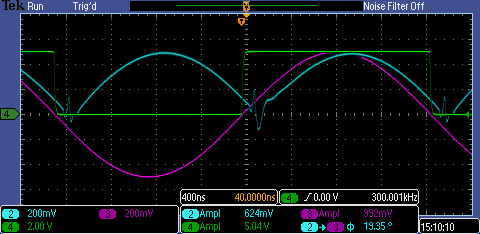
\includegraphics[scale=0.4]{Images/Seance3/partie1/TEK00010.PNG}}
        \caption{$U_{p}$, $U_{mod}'$ et $U_{mult}$ avec un\\ déphasage de 0° à 300 kHz }
    \label{fig:oc21}
    \end{minipage}
    \hfill%
    \begin{minipage}[c]{.50\linewidth}
        \centering
        \rotatebox{0}{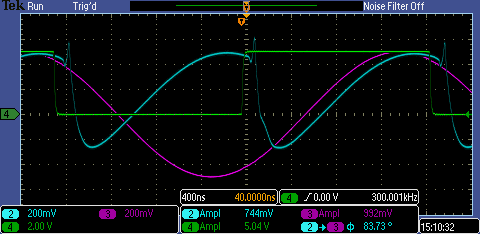
\includegraphics[scale=0.4]{Images/Seance3/partie1/TEK00013.PNG}}
       \caption{$U_{p}$, $U_{mod}'$ et $U_{mult}$ avec un \\ déphasage de 60° à 300 kHz}
 \label{fig:oc22}
    \end{minipage}
\end{figure}

\begin{figure}[H]
    \begin{minipage}[c]{.50\linewidth}
        \centering
        \rotatebox{0}{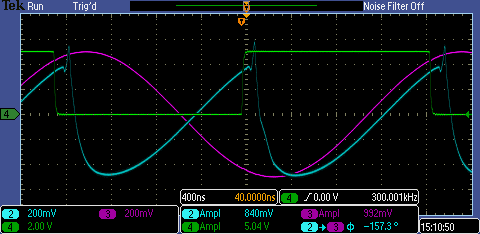
\includegraphics[scale=0.4]{Images/Seance3/partie1/TEK00016.PNG}}
        \caption{$U_{p}$, $U_{mod}'$ et $U_{mult}$ avec un\\ déphasage de 120° à 300 kHz }
    \label{fig:oc23}
    \end{minipage}
    \hfill%
    \begin{minipage}[c]{.50\linewidth}
        \centering
        \rotatebox{0}{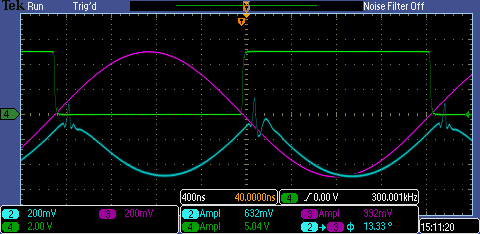
\includegraphics[scale=0.4]{Images/Seance3/partie1/TEK00019.PNG}}
       \caption{$U_{p}$, $U_{mod}'$ et $U_{mult}$ avec un \\ déphasage de 180° à 300 kHz}
 \label{fig:oc24}
    \end{minipage}
\end{figure}

\subsubsection{Analyse}

Les représentations permettent d’observer l’effet du multiplicateur  
décrit au point 4.2.1, puisque le signal \( U_{mult} \) s’inverse lors du passage à zéro du signal carré.  
Cette inversion se produit indépendamment de la valeur du déphasage. \\

Des différences apparaissent toutefois entre les séries de mesures à 100~kHz et à 300~kHz. \\  
À 300~kHz, l’électronique peine à suivre : le signal \( U_{mult} \) est déphasé par rapport au signal \( U_{mod}' \),  
et de fortes aberrations sont visibles lors des flancs du signal \( U_{p} \). \\  
Une fréquence de 300~kHz est donc trop élevée pour ce système, ce qui justifie  
l’utilisation d’une fréquence de 150~kHz pour les manipulations précédentes.


\subsection{Filtrage}

\subsubsection{Représentation des signaux}

Ci-dessous sont représentés les signaux aux différents déphasages relevés à l'oscilloscope. 

\begin{figure}[H]
    \begin{minipage}[c]{.50\linewidth}
        \centering
        \rotatebox{0}{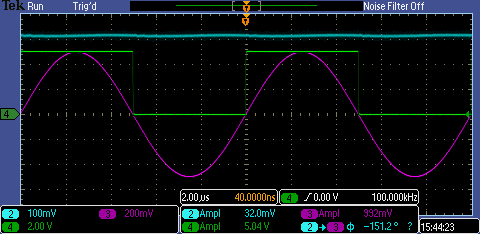
\includegraphics[scale=0.4]{Images/Seance3/partie2/TEK00000.PNG}}
        \caption{Filtre avec RC avec déphasage de 0° }
    \label{fig:f1}
    \end{minipage}
    \hfill%
    \begin{minipage}[c]{.50\linewidth}
        \centering
        \rotatebox{0}{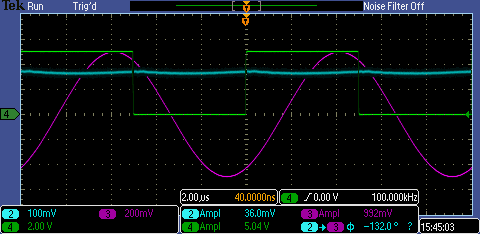
\includegraphics[scale=0.4]{Images/Seance3/partie2/TEK00003.PNG}}
       \caption{Filtre avec RC avec déphasage de 60°}
 \label{fig:f2}
    \end{minipage}
\end{figure}

\begin{figure}[H]
    \begin{minipage}[c]{.50\linewidth}
        \centering
        \rotatebox{0}{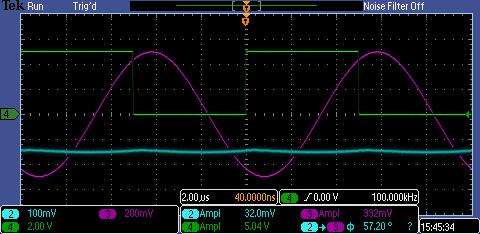
\includegraphics[scale=0.4]{Images/Seance3/partie2/TEK00006.PNG}}
        \caption{Filtre avec RC avec déphasage de 120°}
    \label{fig:f3}
    \end{minipage}
    \hfill%
    \begin{minipage}[c]{.50\linewidth}
        \centering
        \rotatebox{0}{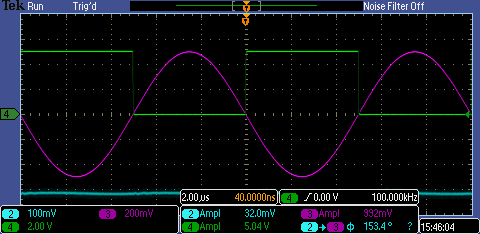
\includegraphics[scale=0.4]{Images/Seance3/partie2/TEK00009.PNG}}
       \caption{Filtre avec RC avec déphasage de 180°}
 \label{fig:f4}
    \end{minipage}
\end{figure}



\subsection{Conclusion}
%\section{Séance 4 - Déphasage et linéarité}
\newpage
\section{Conclusion}

Ces trois premières séances ont permis une première étude du capteur
inductif.

Elles ont permis de :

\begin{itemize}
    \item Déterminer le matériau de la cible du capteur comme étant du cuivre;
    \item Déterminer la fréquence de résonance du circuit de la carte et déterminer la fonction 
    de transfert correspondante, qui s'est avérée correspondre au résultat attendu; 
    \item Décrire et observer le comportement du multiplicateur et du filtre RC. 
\end{itemize}

\textbf{Améliorations :}

Bien que les résultats soient globalement bons, ces trois séances ont eu leurs lots de surprises.
Le capteur initialement utilisé présentait un défaut de câblage ce qui a nécessité une reprise 
complète des mesures de la séance 1 et engendré un certain retard. Une erreur d'anticipation et  
une réaction trop lente de notre part qui aurait pu être évitée.




\begin{thebibliography}{9}

    \bibitem{donneelabo}
    Demierre, Michel
    \textit{Cours : mini-projet : séances 1,2,3},
    [ HEIG-VD Capteurs]
    
    \bibitem{cours}
    Demierre, Michel
    \textit{Cours : Suopport de cours },
    [ HEIG-VD Capteurs]
    
    
    \end{thebibliography}



\begin{flushright}
    Yverdon, {\today\par}
\end{flushright}
% \vspace{1cm}

\begin{figure}[H]
    \centering
    \begin{minipage}[b]{0.3\textwidth}
      \centering
      Bianchi Romain\\
      
\includegraphics[height=0.4\textwidth]{Images/Bianchi.jpg}
    \end{minipage}
    \hfill
    \begin{minipage}[b]{0.3\textwidth}
      \centering
      Larghi Andrea\\
      \includegraphics[height=0.4\textwidth]{logos/arbre.png}
    \end{minipage}
  \end{figure}

\newpage
\printbibliography % To generate the bibliography


\newpage
\appendix

% \includepdf[pages=1,pagecommand={\thispagestyle{empty}\vspace*{-3.3cm}\section{SKF 618/4}\label{pdf:skf 618_4}}]{PDF/Louis/618_4 SKF.pdf}
\includepdf[pages=1-11]{PDF/projet_capteur.pdf}

\end{document}
